\documentclass[12pt]{article}
\usepackage{fullpage}
\usepackage{subcaption,amsmath,amssymb,mathtools,xparse,graphicx,float,datetime,color,array,graphics,enumerate,tikz,pgfplots,xcolor}
\usepgfplotslibrary{statistics}
\pagestyle{empty}
\newcommand{\D}{\displaystyle}
\setlength{\textheight}{9in} \setlength{\headheight}{.2in}
\setlength{\headsep}{0in} \setlength{\topmargin}{0in}
\begin{document}
\begin{center}
CSCI 6100 Machine Learning From Data\\
Fall 2018\\
\end{center}
\begin{center}
HOMEWORK 10\\
Daniel Southwick\\
661542908\\
southd@rpi.edu
\end{center}
\vspace{.1in}

\noindent {\bf Exercise 6.1} \\\\
a)\\\\
\indent High cosine similarity but low Euclidean distance similarity $u = \left[ 1, 0 \right]$, $v = \left[ 10, 0 \right]$:\\
\begin{align*} 
\mbox{CosSim}( {u},  {v}) &= \frac{ {u}\cdot {v}}{\| {u}\|\| {v}\|} = \frac{10}{10} = 1 \indent
d( {u},  {v}) = \| {u}-  {v}\| = 10 - 1 = 9
\end{align*}
\indent Low cosine similarity but high Euclidean distance similarity $u = \left[ 0.1, 0 \right]$, $v = \left[ -0.1, 0 \right]$:\\
\begin{align*} 
\mbox{CosSim}( {u},  {v}) &= \frac{ {u}\cdot {v}}{\| {u}\|\| {v}\|} = \frac{-0.01}{0.1\times0.1} = -1  \indent
d( {u},  {v}) = \| {u}-  {v}\| = 0.1 + 0.1 = 0.2 
\end{align*}
b)\indent If the origin of the coordinate system changes, the coordinate values of $u$ and $v$ will change, the relative distance between $u$ and $v$ will always be the same, so $CosSim(u,v)$ changes while $d(u,v)$ stays the same. Thus, Euclidean distance 
should be chosen instead of cosine similarity as the new feature.\\\\

\noindent {\bf Exercise 6.2} \\\\
a) To show $e(f( {x})) = \mathbb{P}[f( {x})\neq y] = \min\{\pi( {x}), 1-\pi( {x})\}$ ($\pi( {x}) = \mathbb{P}[y=+1\big| {x}]$): \\\\
\indent If $\pi( {x}) \geq \frac{1}{2}$, Then choose $f( {x}) = +1$ and the Probability of error is:\\ 
$\quad \min\{\pi( {x}), 1-\pi( {x})\} = 1-\pi( {x})$\\\\
\indent If $\pi( {x}) < \frac{1}{2}$, Then choose $f( {x}) = -1$, and the Probability of error is:\\ 
$\quad \min\{\pi( {x}), 1-\pi( {x})\} = \pi( {x})$\\\\
\indent So $e(f( {x})) = \mathbb{P}[f( {x})\neq y] = \min\{\pi( {x}), 1-\pi( {x})\}$\\\\
b) To show $e(f( {x}))\leq e(h( {x}))$  for any other hypothesis $h$: \\\\
\indent Since there are only two outcomes of $f(x)$, $+1$ and $-1$. We let $f(x) = +1$ if $\pi(x) \geq p$, thus $f(x) = -1$ otherwise. Then for any test point $x$, the probability error became: $\pi(x) = p\times (1-p) + (1-p)\times p = -2p^2 + 2p = 2p*(1-p)$, so the minimum of $\pi(x)$ is where $p = \frac{1}{2}$. Thus $e(f( {x}))\leq e(h( {x}))$.

\newpage
\noindent {\bf Problem 6.1} \\\\
a) The decision regions for the 1-NN and k-NN are shown below, the red region denotes class -1 and the black region denotes class +1 and the figures are shown in the range from $\left[-2, 2\right]$ for both x and y:
\begin{figure}[H]
\centering
\begin{subfigure}{.5\textwidth}
  \centering
   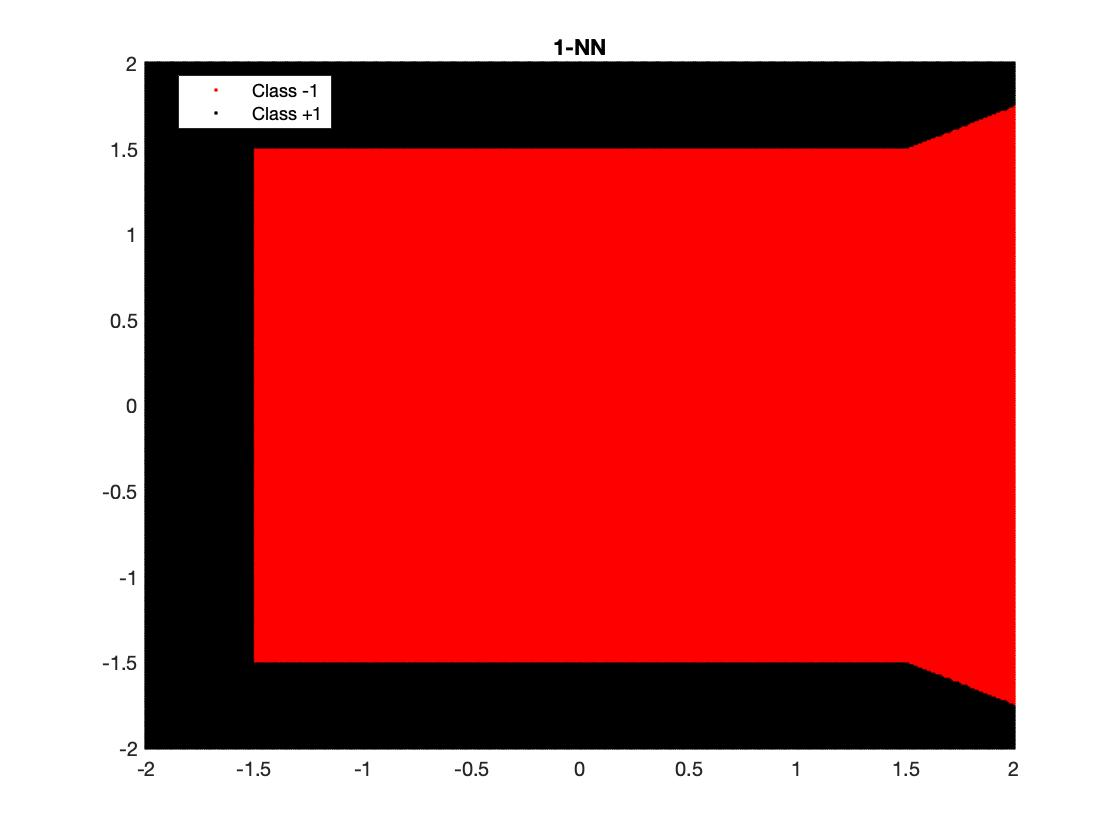
\includegraphics[scale = 0.22]{1.jpg}
  \caption{1-NN Classification}
  \label{fig:1}
\end{subfigure}%
\begin{subfigure}{.5\textwidth}
  \centering
   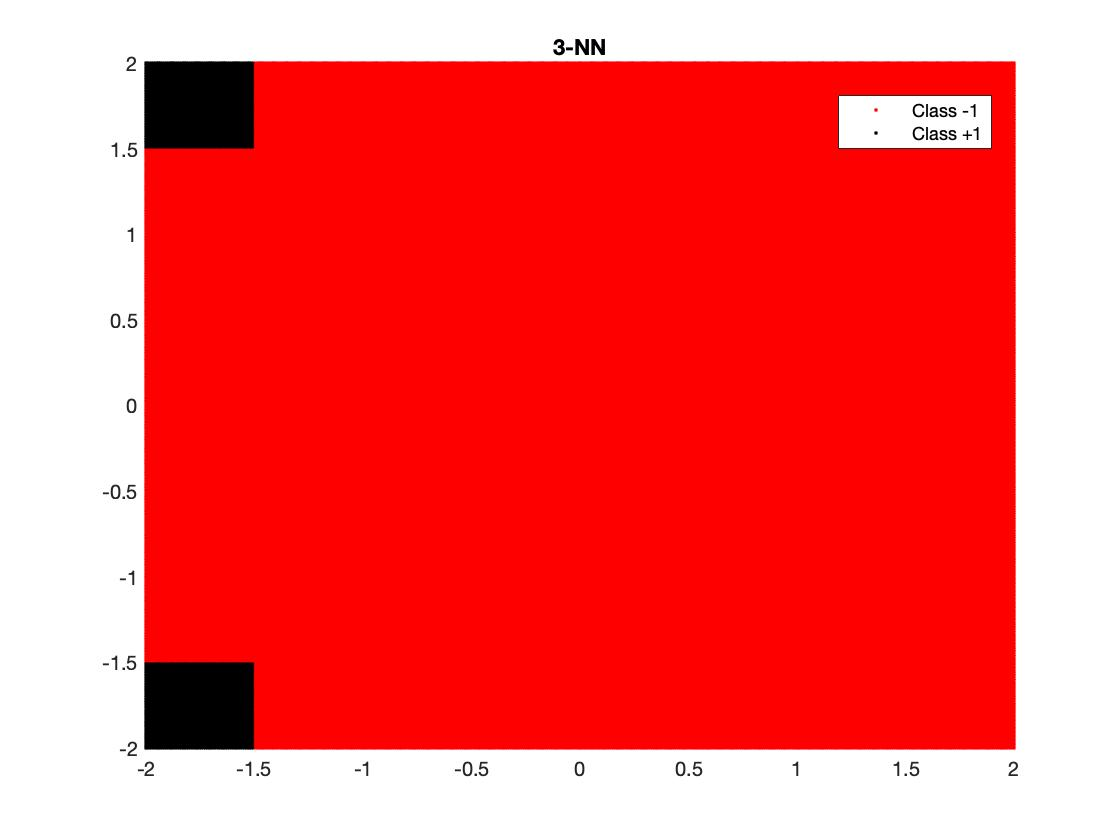
\includegraphics[scale = 0.22]{2.jpg}
  \caption{3-NN Classification}
  \label{fig:2}
\end{subfigure}
\caption{Non-Transformed Nearest Neighbor(s) Classification}
\label{fig:test}
\end{figure}
b) The decision regions for the transformed 1-NN and k-NN are shown below, the red region denotes class -1 and the black region denotes class +1 and the figures are shown in the range from $\left[-2, 2\right]$ for both x and y:
\begin{figure}[H]
\centering
\begin{subfigure}{.5\textwidth}
  \centering
   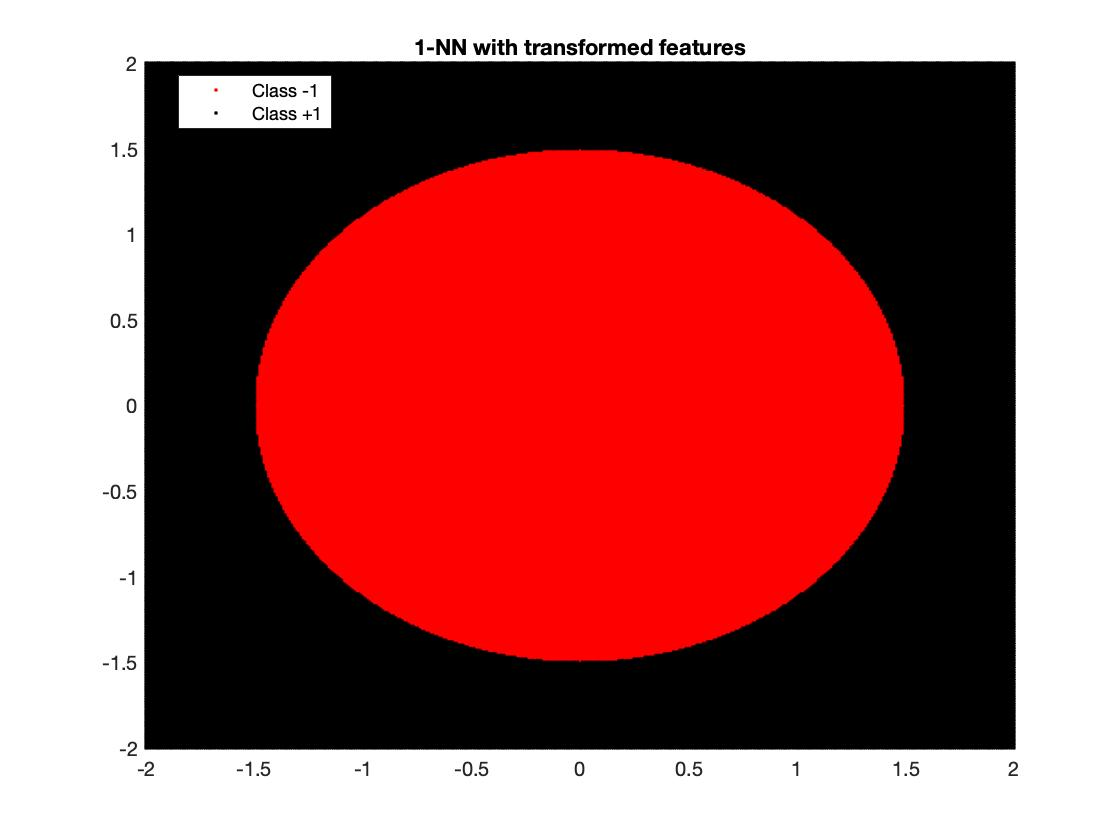
\includegraphics[scale = 0.22]{3.jpg}
  \caption{1-NN Transformed Classification}
  \label{fig:3}
\end{subfigure}%
\begin{subfigure}{.5\textwidth}
  \centering
   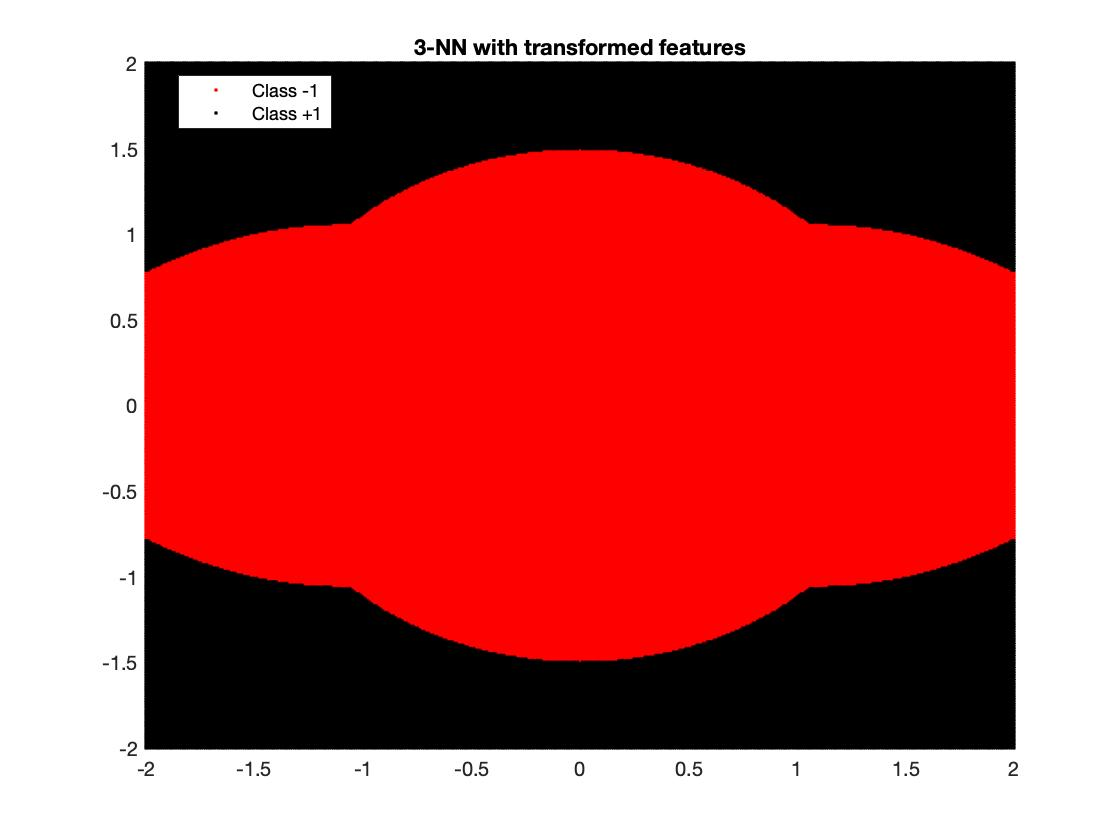
\includegraphics[scale = 0.22]{4.jpg}
  \caption{3-NN Transformed Classification}
  \label{fig:4}
\end{subfigure}
\caption{Transformed Nearest Neighbor(s) Classification}
\label{fig:test}
\end{figure}

\newpage
\noindent {\bf Problem 6.4} \\\\
\indent We revisit Problem 3.1 and generated 2000 data points:
\begin{figure}[H]
  \centering
  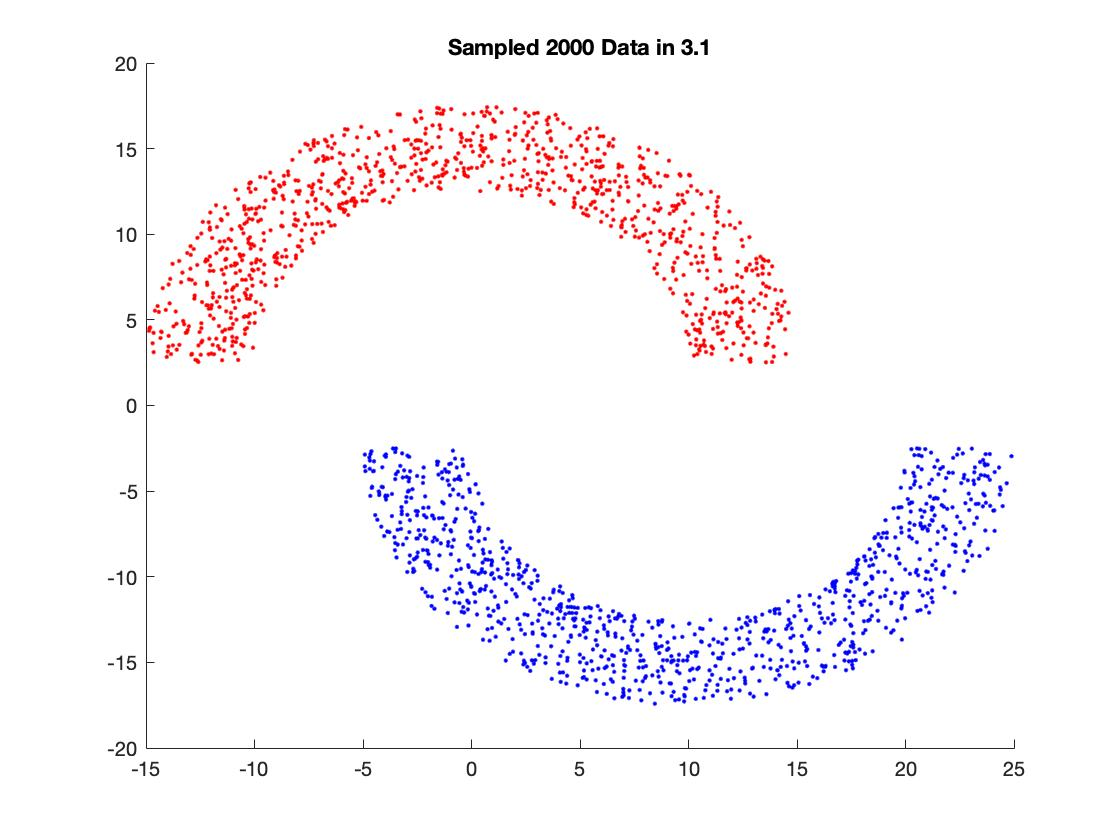
\includegraphics[scale = 0.3]{5.jpg}
  \caption{Data Points Generated Using 3.1}
  \label{fig:5}
\end{figure}
\indent The 1-NN and 3-NN Classification are listed below, where the red/blue region corresponded to the red/blue data point generated above, there's not much a difference between 1-NN and 3-NN as the dataset is large and separable.
\begin{figure}[H]
\centering
\begin{subfigure}{.5\textwidth}
  \centering
   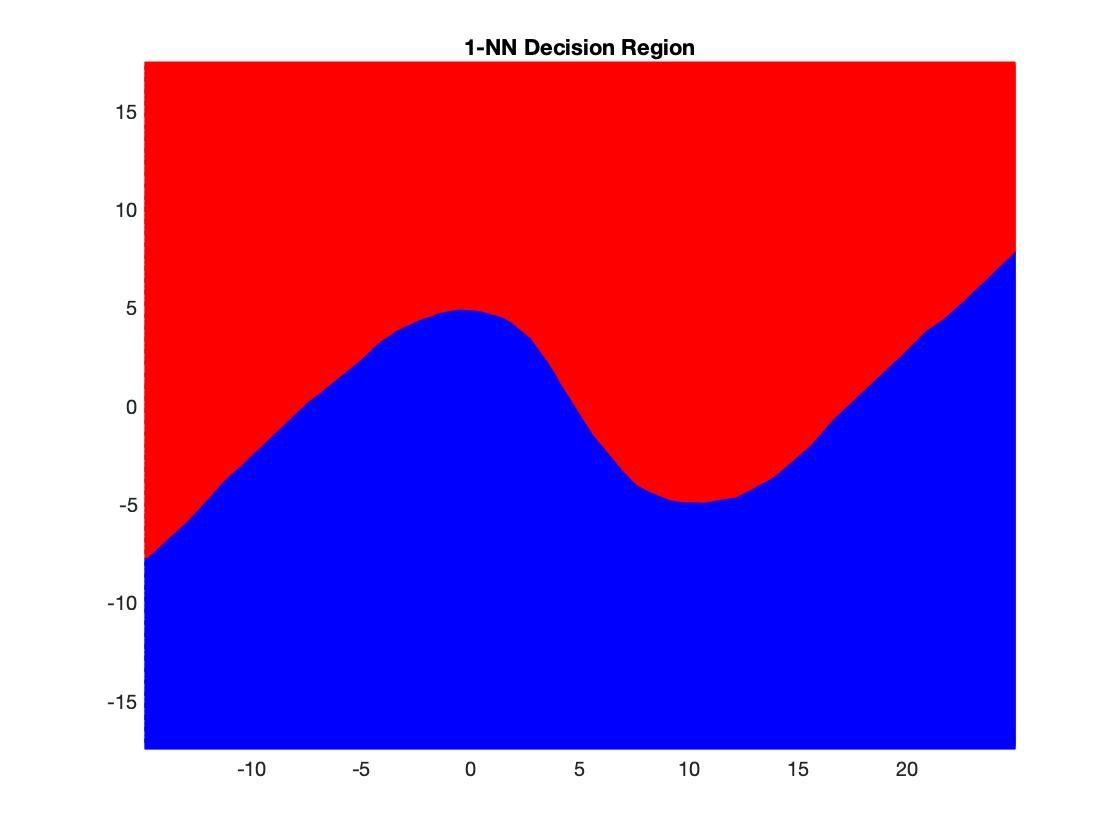
\includegraphics[scale = 0.22]{6.jpg}
  \caption{1-NN Classification}
  \label{fig:6}
\end{subfigure}%
\begin{subfigure}{.5\textwidth}
  \centering
   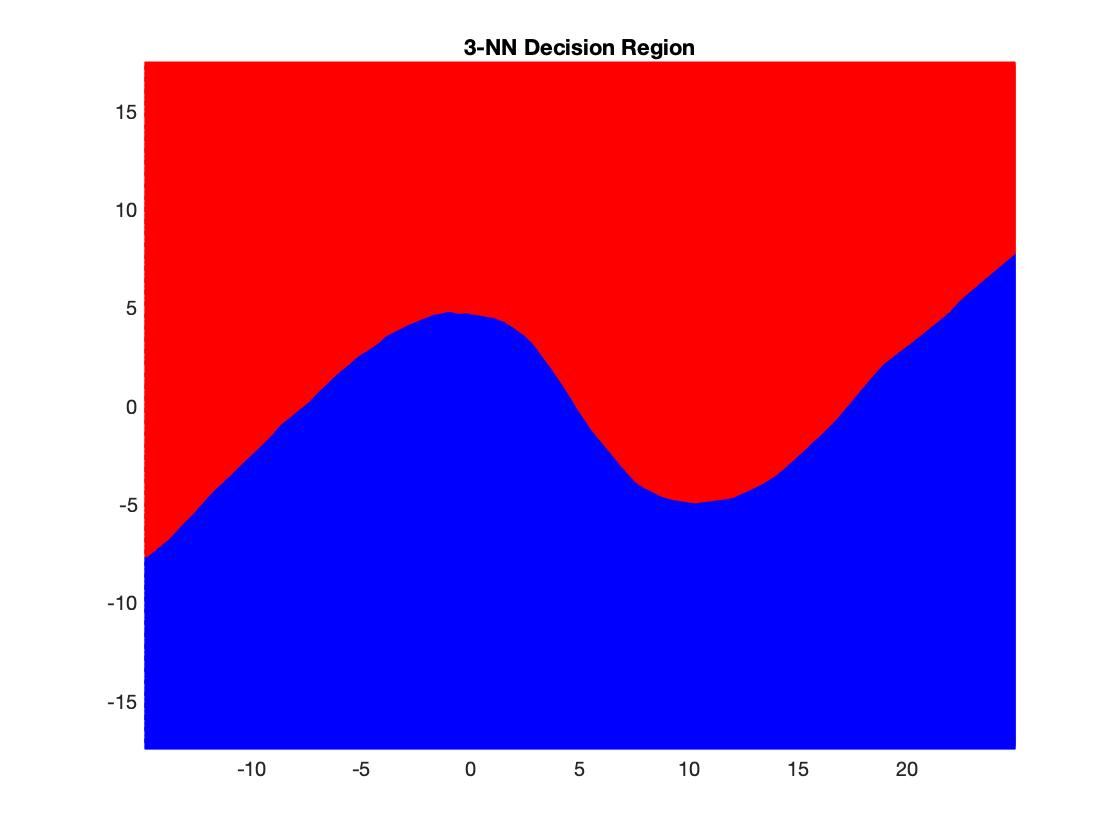
\includegraphics[scale = 0.22]{7.jpg}
  \caption{3-NN Classification}
  \label{fig:7}
\end{subfigure}
\caption{Nearest Neighbor(s) Classification for 3.1}
\label{fig:test}
\end{figure}

\newpage
\noindent {\bf Problem 6.16} \\\\
a)\\
\indent i) We first randomly generated 10,000 data in the unit square $\left[ 0, 1\right]^2$. Then, we initially select 10 centers using the simple greedy heuristic method described in the text, then we updated these centers using Lloyd's algorithm, the results are as follows:
\begin{figure}[H]
\centering
\begin{subfigure}{.5\textwidth}
  \centering
   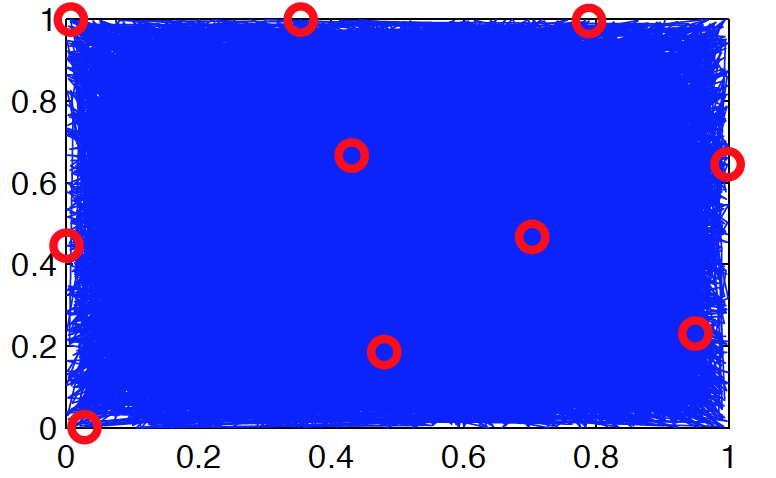
\includegraphics[scale = 0.5]{8.jpg}
  \caption{Simple Greedy Heuristic Center}
  \label{fig:8}
\end{subfigure}%
\begin{subfigure}{.5\textwidth}
  \centering
   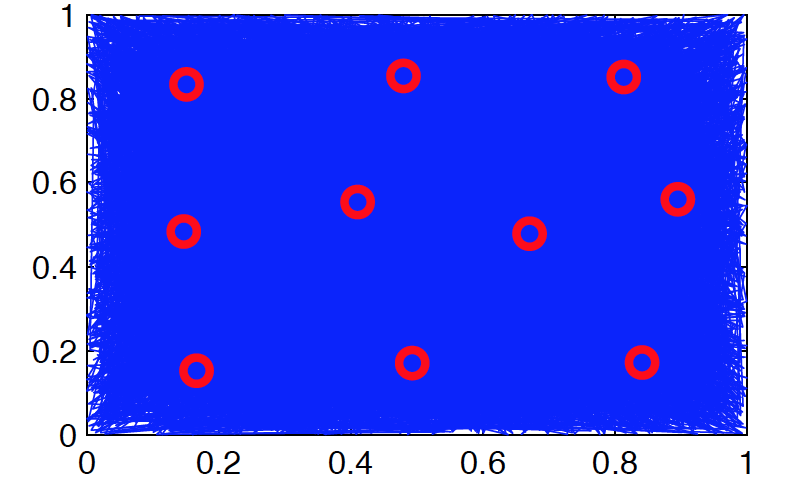
\includegraphics[scale = 0.5]{9.jpg}
  \caption{Lloyd's Updated Center}
  \label{fig:9}
\end{subfigure}
\caption{10 Centers of the 10,000 Data}
\label{fig:test}
\end{figure}
\indent ii) We then generate 10,000 query points and compare the running time of brute force approach and the branch and bound method. In here, we used Matlab's tic/toc command, it took about 6.92 seconds for brute force and only about 2.19 seconds for the branch and bound method to determine the nearest neighbors of the generated 10,000 query data. The branch and bound method is a little bit over three times faster than the brute force. \\\\
b)\\
\indent i) Same as part a), but this time we generated 10 Gaussians with center's randomly distributed in $\left[ 0, 1\right]^2$, with individual variance $\sigma = 0.1$ and each Gaussian is independent of each other. Again, we initially select 10 centers using the simple greedy heuristic method described in the text, then we updated these centers using Lloyd's algorithm, the results are as follows:
\begin{figure}[H]
\centering
\begin{subfigure}{.5\textwidth}
  \centering
   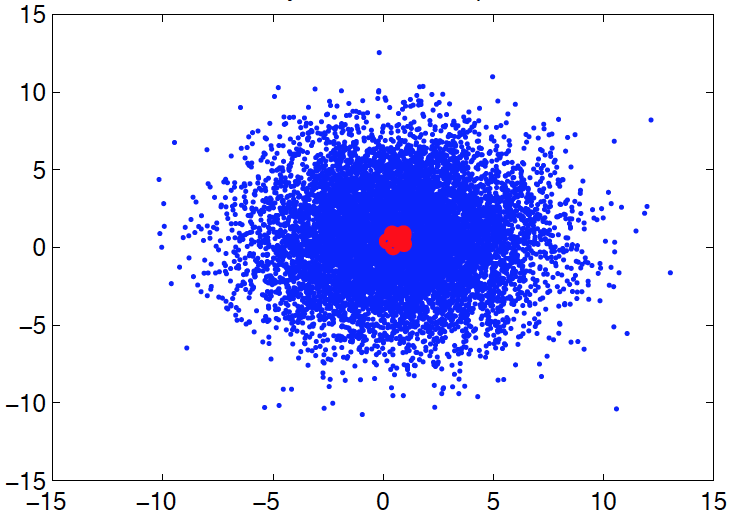
\includegraphics[scale = 0.5]{10.jpg}
  \caption{Simple Greedy Heuristic Center}
  \label{fig:8}
\end{subfigure}%
\begin{subfigure}{.5\textwidth}
  \centering
   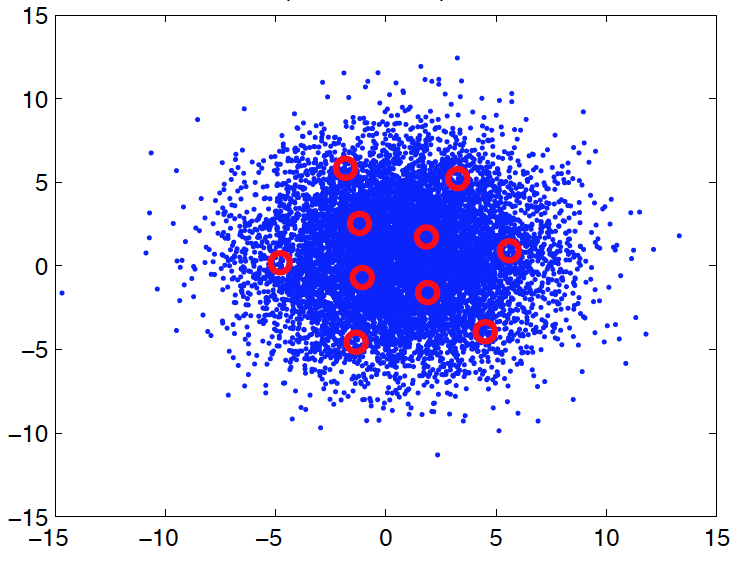
\includegraphics[scale = 0.5]{11.jpg}
  \caption{Lloyd's Updated Center}
  \label{fig:9}
\end{subfigure}
\caption{10 Centers of 10 Gaussian Mixture}
\label{fig:test}
\end{figure}
\indent ii) Again, We then generate 10,000 query points and compare the running time of brute force approach and the branch and bound method. Using Matlab's tic/toc command, this time, it took about 7.60 seconds for the brute force method and about 5.84 seconds for the branch and bound method. The branch and bound method is still faster than the brute force but not as significant as part a).\\\\
c)\\
\indent The branch and bound method is faster than the brute force approach for either cases above, and it will always be faster. Since for the branch and bound method, some of the query data points can be categorized by computing the distance with only part of the training data, however, for the brute force method, The distance between all query data points and all training data points needs to be computed in order to make the decision. Thus it takes more time.\\
d)\\
\indent No, it does not depend on the number of test points, branch and bound method should always be better than the brute force method by the nature of the algorithm.
\end{document}

